\documentclass[12pt]{article}
\usepackage{graphicx}
\usepackage{hyperref}
\usepackage{enumerate}
\usepackage{supertabular}
\usepackage{verbatim}
%\usepackage{fullpage}
\usepackage[margin=2.5cm]{geometry}

\begin{document}

%titlepage
\begin{titlepage}
\title{Tanks}
\author{McKinley Olsen}
\date{\today}
\maketitle
\end{titlepage}

%TABLE OF CONTENTS
\newpage
\tableofcontents
\newpage

\section{Functional Requirements}

\begin{enumerate}

	\item{A player can register or unregister themselves with the fight manager at any time.}
	
	\item{A player can move around in a physical space, as long as the following constraints are observed:}
	\begin{enumerate}
		\item{The rate (distance / time) at which a player can move is limited.}
		\item{A player cannot move if they are trying to get a shell from the Shell Manager, or are filling a shell with the Gunpowder Manager.}
		\item{A player that violates these constraints is removed from all fights and unregistered with the Fight Manager}
	\end{enumerate}
	
	\item{A player can fire non-empty shells at any player.}
	\begin{enumerate}
		\item{The Fight Manager can broadcast a fired shell's location to all players. Every player at that location must reply back that they were hit.}
		\item{If a player responds that they were hit, but took longer than 10ms to reply to the Fight Manager, the Fight Manager will remove that player from all games and de-register them.}
		\item{A player that fires and hits another player that is not participating in any of the games that player is participating creates a new fight. }
	\end{enumerate}
	
	\item{A player can ask the Fight Manager for a list of a player’s most recent known locations (up to 10).}
	\begin{enumerate}
		\item{The Fight Manager can request the last 10 locations from a player, and the player will respond with their last 10 locations.}
		\item{If the response of a player with their locations takes longer than 10ms, the Fight Manager will remove that player from all games and de-register them. }
	\end{enumerate}
	
	\item{A player can ask the Fight Manager for a list of current players.}
	\begin{enumerate}
		\item{Players can also ask the Fight Manager for a list of players in a specific fight.}
	\end{enumerate}
	
	\item{A player can instigate a fight at any time, regardless of what other fights are in progress.}
	\begin{enumerate}
		\item{A player instigates a fight by telling the fight manager that it is launching a shell (filled with some percentage of gunpowder) at a player that is believed to be at a specified location.}
		\item{If the location of the other player was correct, then the player is “hit” with the shell and the fight begins.}
		\item{The instigator and the player hit with the shell are automatically enrolled in the new fight.}
	\end{enumerate}
	
	\item{Players can join fights in progress at any time.}
	\begin{enumerate}
		\item{Players can request a list of in progress fights from the fight manager.}
	\end{enumerate}
	
	\item{Players do not have to take turns when fighting; they are able to perform an action they choose at any time, so long as the action is in accordance with the aforementioned restrictions.}
	
	\item{Players can request an empty shell from the shell manager, but only hold up to 4 shells at a time.}
	
	\item{A player can fill an empty shell by making a request to the gun powder manager to fill the shell to a specified percentage.}
	
	\item{Once a player has been hit with shell(s) that contained an accumulated 100 or more cups of gunpowder, the player is removed from all fights and de-registered.}
	
	\item{A fight manager must be able to update a SOAP webservice with information about itself and the game}
	\begin{enumerate}
		\item{The manager must provide the following information when started, which should be easily specifiable before starting the manager:}
		\begin{enumerate}
			\item{The URL of the webservice}
			\item{A name for the manager}
			\item{The name of the person operating the manager}
			\item{The e-mail address of the person operating the manager}
			\item{A global unique identifier (GUID) to identify the manager}
		\end{enumerate}
		\item{The manager must inform the webservice when a new fight is started, providing to it the id of the fight and the manager's GUID}
		\item{The manager must update the webservice on the current state of the game periodically. This should include information such as:}
		\begin{enumerate}
			\item{The time the update message was sent}
			\item{The current status of the game}
			\item{The current number of players}
			\item{The maximum number of players that have played}
			\item{The number of shells that have been launched in the game}
			\item{The amount of gunpowder that has been launched}
			\item{The amount of shells that hit players}
			\item{The amount of gunpowder that hit players}
			\item{The name of the winning player, if the game has been won}
		\end{enumerate}
	\end{enumerate}
\end{enumerate}

\section{Protocols}
	\subsection{Introduction}
		This section describes the protocols required in order to communicate between processes in Virtual Tanks.
	
	\subsection{Overview}
		Detailed below are the protocols used in the Virtual Tanks and their important characteristics. The communication patterns utilized are as follows:
		\begin{itemize}
			\item{Request-Reply: a two-way communication from initiator to receiver(s), and from receiver(s) to initiator. As a reply message is communicated by the receiver(s), this pattern is generally considered reliable.}
			\item{Custom: A non-standard sequence of messages is used for this protocol. The sequence of messages will be described later in the document.}
		\end{itemize}
		
		\tablehead{\hline \textbf{Protocol} & \textbf{Description} & \textbf{Initiator} & \textbf{Other Components Involved} & \textbf{Communication Pattern} \\ \hline}
		\begin{center}
		    \begin{supertabular}{|p{2cm}|p{5cm}|p{2cm}|p{2.5cm}|l|}
		        \hline
		        	%REQUIREMENT #1
		        	Register & Allows a player to register with the Fight Manager, making them visible to other players and managed by the Fight Manager. Initiated when a player wishes to begin playing the game.& Player & Fight Manager & Request-Reply \\ \hline
		        	Unregister & Allows a player to unregister from all games and to have that player become unknown to the Fight Manager. This protocol is initiated when the player wishes to quit, when a general application error occurs, or initiated by the Fight Manager when the player has met or exceeded the number of cups of gunpowder it takes to lose (specified in requirement 13), or when a player takes more than 10ms to respond to a Shell Fired Request.& Player, Fight Manager & Fight Manager, Player & Request-Reply \\ \hline
		        
		        	%REQUIREMENT #3
		        	Fire Shell & Allows a player to fire a shell filled with gunpowder at a location. This request is sent to the Fight Manager, who then proceeds to broadcast the shell's location to all players, who in turn only respond if they were effected by the shell.& Player & Fight Manager, Players & Custom \\ \hline
		        
		        	%REQUIREMENT #4
		        	Location List & Allows a player to be informed of the up to 10 most recent locations of another player. Initiated when the player wishes to know the whereabouts of another player.& Player & Fight Manager, Specified Player & Custom \\ \hline
		        	
		        	%REQUIREMENT 5
		        	Player List &  Allows a player to either get a list of all the players currently registered, or all the players in a specified fight. Initiated when the player wishes to know about other players.& Player & Fight Manager & Custom \\ \hline
		        	
		        	%REQUIREMENT #6
		        	Create Fight & Allows a player to create a new fight. Initiated when a player fires upon and hits a player that is not currently participating in any of the fights the firing player is participating in. & Player & Fight Manager & Custom \\ \hline
		        	
		        	%REQUIREMENT #7
		        	Join Fight & Allows a player to enlist/delist to a fight. A player requesting to register for a fight they are not currently enlisted in joins the fight. Conversely, a player requesting to register for a fight they are currently enlisted in leaves the fight. & Player & Fight Manager & Request-Reply \\ \hline
						Fight List & Allows a client to be informed of the currently active fights. Initiated when the player wishes to see available fights.& Player & Fight Manager & Custom \\ \hline
		        	
		        	%REQUIREMENT #9
		        	Get Shell & Allows a player to request an empty shell from the Shell Manager. As specified in the requirements, a player may have up to 4 empty or non-empty shells at a time. Initiated when the player wishes to get a new shell.& Player & Shell Manager & Request-Reply \\ \hline
		        	%REQUIREMENT #10
		        	Fill Shell & Allows a player to fill an empty shell to a specified percentage. Initiated by the player when they wish to prepare a shell for firing.& Player & Gunpowder Manager & Request-Reply \\ \hline
				\hline
		    \end{supertabular}
		\end{center}
		
\section{Message Types and their Definitions}
		\subsection{Introduction}
			Described here is the structure of the messages required to implement the aforementioned protocols. The structure is conveyed through class diagrams. These class diagrams omit certain methods, such as the constructor, getters/setters, create, encode, and decode. These methods are implied in the following diagrams, as their definition is relatively unimportant.
		\subsection{Diagrams}
			\newpage
			\subsubsection{General Message Classes}
				\begin{center}
					\begin{figure}[htp]
						\centering
						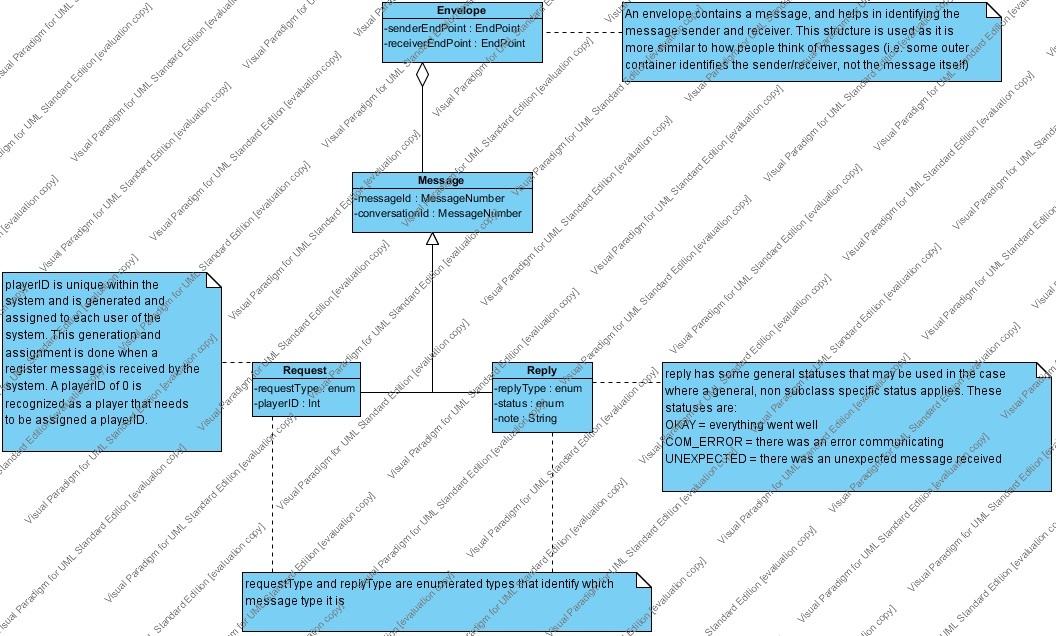
\includegraphics[width=\textwidth]{Diagrams/Class Diagrams/Message Classes.jpg}
						\caption{The general superclasses used. All remaining classes inherit from these.}
					\end{figure}
				\end{center}
			\newpage
			\subsubsection{Register Protocol}
				\begin{center}
					\begin{figure}[htp]
						\centering
						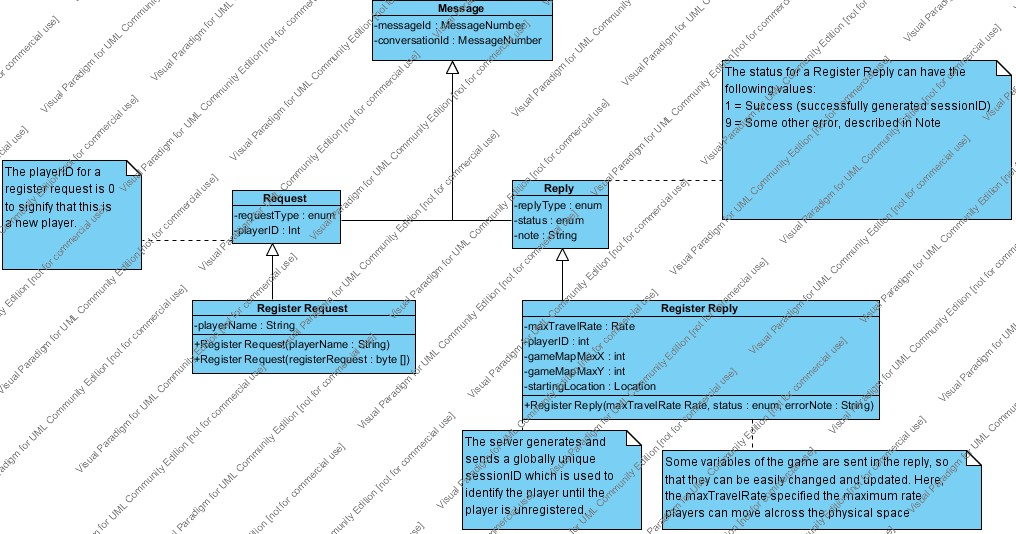
\includegraphics[width=\textwidth]{Diagrams/Class Diagrams/Register Protocol.jpg}
						\caption{The message classes used in the Register Protocol}
					\end{figure}
				\end{center}
			\newpage
			\subsubsection{Unregister Protocol}
				\begin{center}
					\begin{figure}[htp]
						\centering
						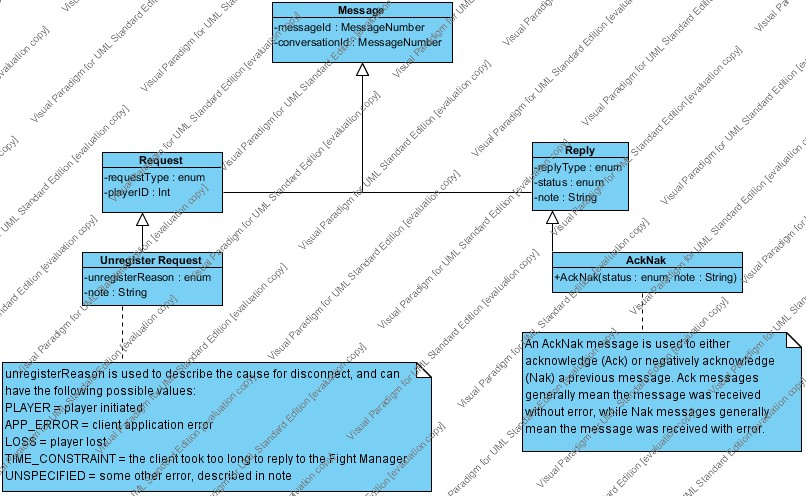
\includegraphics[width=\linewidth]{Diagrams/Class Diagrams/Unregister Protocol.jpg}
						\caption{The message classes used in the Unregister Protocol}
					\end{figure}
				\end{center}
			\newpage
			\subsubsection{Location List Protocol}
				\begin{center}
					\begin{figure}[htp]
						\centering
						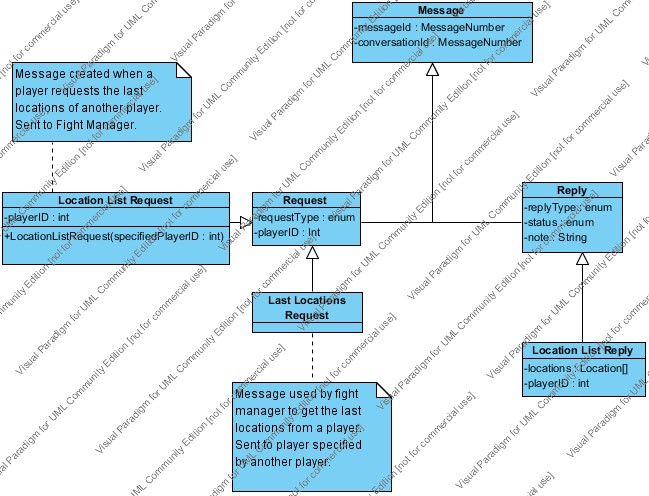
\includegraphics[width=\textwidth]{Diagrams/Class Diagrams/Location List Protocol.jpg}
						\caption{The classes used in the Location List Protocol}
					\end{figure}
				\end{center}
			\newpage
			\subsubsection{Player List Protocol}
				\begin{center}
					\begin{figure}[htp]
						\centering
						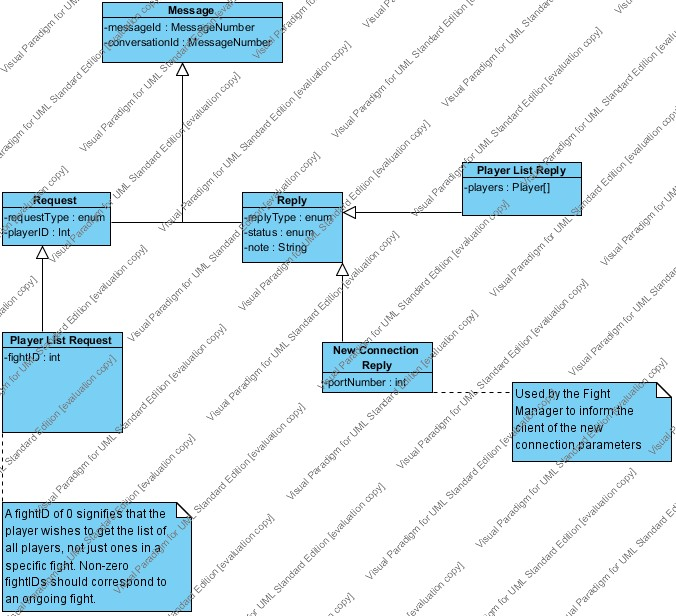
\includegraphics[width=\textwidth]{Diagrams/Class Diagrams/Player List Protocol.jpg}
						\caption{The classes used in the Player List Protocol}
					\end{figure}
				\end{center}
			\newpage
			\subsubsection{Fight List Protocol}
				\begin{center}
					\begin{figure}[htp]
						\centering
						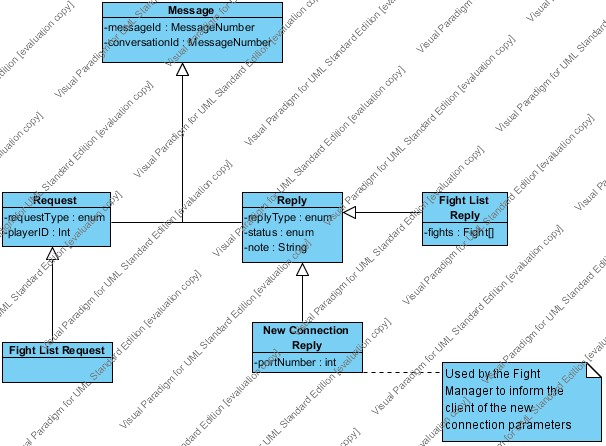
\includegraphics[width=.8\textwidth]{Diagrams/Class Diagrams/Fight List Protocol.jpg}
						\caption{The classes used in the Fight List Protocol}
					\end{figure}
				\end{center}
			\newpage
			\subsubsection{Join Fight Protocol}
				\begin{center}
					\begin{figure}[htp]
						\centering
						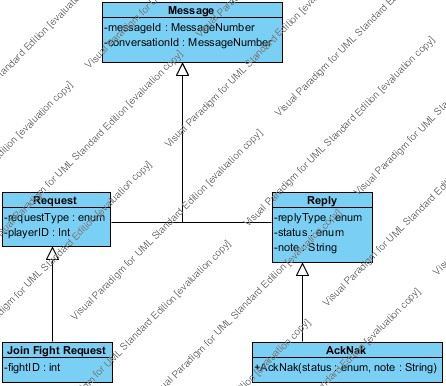
\includegraphics[width=.7\textwidth]{Diagrams/Class Diagrams/Join Fight Protocol.jpg}
						\caption{The classes used in the Join Fight Protocol}
					\end{figure}
				\end{center}
			\newpage
			\subsubsection{Create Fight Protocol}
				\begin{center}
					\begin{figure}[htp]
						\centering
						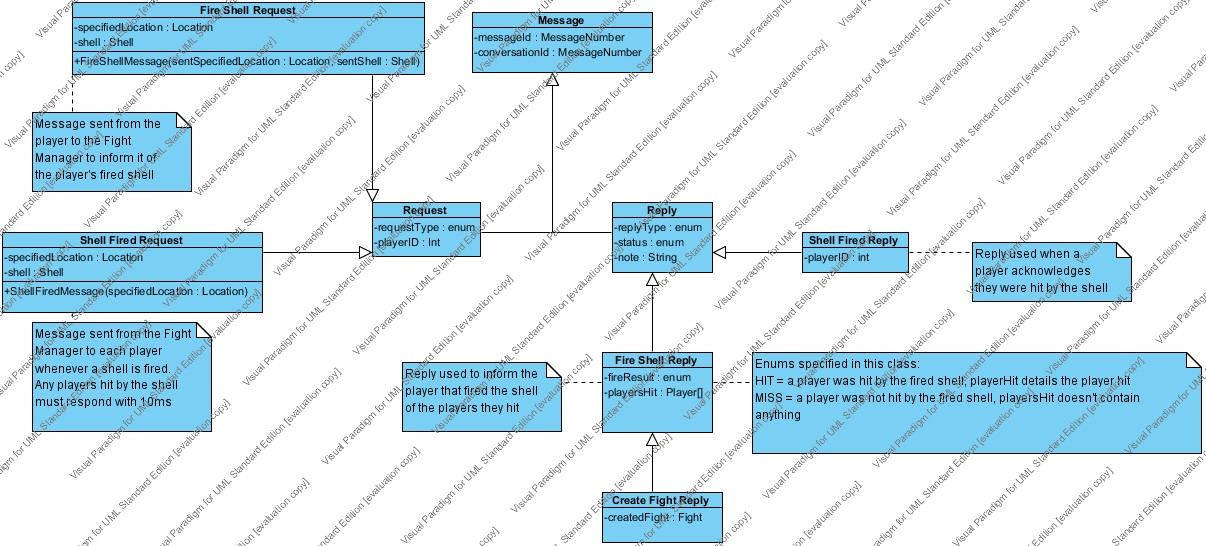
\includegraphics[width=\textwidth]{Diagrams/Class Diagrams/Create Fight Protocol.jpg}
						\caption{The classes used in the Create Fight Protocol}
					\end{figure}
				\end{center}
			\newpage
			\subsubsection{Fire Shell Protocol}
				\begin{center}
					\begin{figure}[htp]
						\centering
						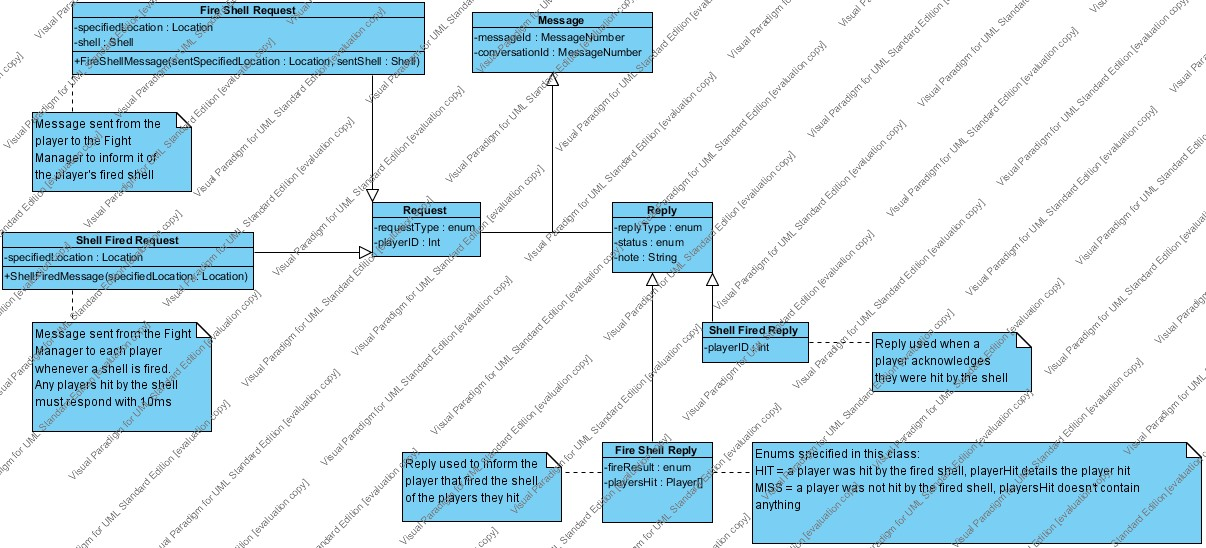
\includegraphics[width=\textwidth]{Diagrams/Class Diagrams/Fire Shell Protocol.jpg}
						\caption{The classes used in the Fire Shell Protocol}
					\end{figure}
				\end{center}
				\newpage
				\subsubsection{Fill Shell Protocol}
					\begin{center}
						\begin{figure}[htp]
							\centering
							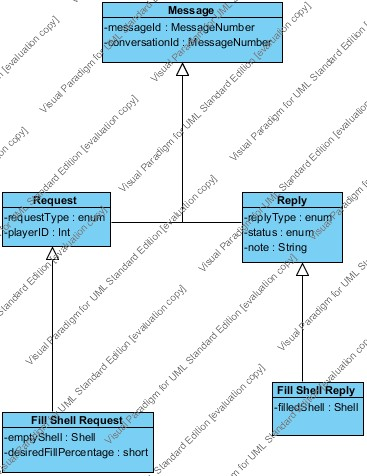
\includegraphics[width=.7\textwidth]{Diagrams/Class Diagrams/Fill Shell Protocol.jpg}
							\caption{The classes used in the Fill Shell Protocol}
						\end{figure}
					\end{center}
				\newpage
				\subsubsection{Get Shell Protocol}
					\begin{center}
						\begin{figure}[htp]
							\centering
							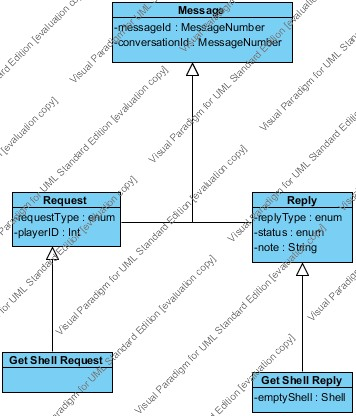
\includegraphics[width=.7\textwidth]{Diagrams/Class Diagrams/Get Shell Protocol.jpg}
							\caption{The classes used in the Get Shell Protocol}
						\end{figure}
					\end{center}
				\newpage
		\subsection{Message Descriptions}
		Note:
		A value in the Valid Attribute Values section that begins with an uppercase letter is a custom object used in the game that, as of yet, has not been fully specified.
			\tablehead{\hline \textbf{Name} & \textbf{Description} & \textbf{Uses} & \textbf{Valid Attribute Values} \\ \hline}
			
			\begin{supertabular}{|p{2cm}|p{5cm}|p{3cm}|p{4cm}|}
				%REGISTER PROTOCOL
				Register Request & Intended to be used when a client needs to register with the Fight Manager. This message is used to notify the Fight Manager of a new player that must be assigned a player ID. & Register Protocol & playerName: "John Smith" \\ \hline
				Register Reply & Sent in reply to a Register Request, a client receiving this message knows they have been registered with the Fight Manager, assigned a unique player ID, and are available to be fired upon. & Register Protocol & playerID: 1 \\&&& rate: Rate \\&&& gameMapMaxX: 100 \\&&& gameMapMaxY: 100 \\&&& startingLocation: Location \\ \hline
				
				%UNREGISTER PROTOCOL
				Unregister Request & Means that a player will be unregistered with the Fight Manager, and that their communication will break. Used when the player quits the game, used by the Fight Manager to inform a player of their forced disconnect. & Unregister protocol & unregisterReason: UNSPECIFIED \\ &&&note:``System Restart" \\ \hline
				
				%FIRE SHELL
				Fire Shell Reply & Used to inform a player of the effect of their shell fire. Means the shell fire of the player was received successfully and that its effects have been noted. & Fire Shell Protocol & fireResult: HIT \\&&&playersHit: Player[]\\ \hline
				
				%LOCATION LIST
				Location List Request& Used when a player instigates a request for a another player's last locations. Means the Fight Manager must query the specified player and find out their last locations.& Location List Protocol&specifiedPlayerID: 1\\ \hline
				Last Locations Request&Used when the Fight Manager needs to ask a player their last locations. Means the player must know and gather their last locations to send back.&Location List Protocol&N/A\\ \hline
				Location List Reply&Used when a player responds to a Last Locations Request and sends back their previous locations. Means the Fight Manager has the information the player requested with the Location List Request, and can send this message onto the player that requested the information.&Location List Protocol&locationList: Location[]\\ \hline
				
				%PLAYER LIST
				Player List Request&Used when a player requests a list of current players. Specifying a fight ID of 0 denotes a request for a list of all players, specifying a valid fight ID denotes a request for a list of players in that fight. Means the Fight Manager must put together a list of either all players or players in a specific fight and send that list back.&Player List Protocol&fightID: 0\\ \hline
				Player List Reply&Used when the Fight Manager needs to send a list of players to the player that requested the list. This message is special, in that it is sent over a TCP connection created to transfer it. To the player, the receipt of this message means the created TCP connection may now be closed.&Player List Protocol&players: Player[]\\ \hline
				
				%CREATE FIGHT
				Fight Creation Reply&Used when a player fired a shell at a location that effected another player that was not in any of the fights they were participating. Means a new game has been created that the player is now enrolled in.&Create Fight Protocol&createdFight: Fight\\ \hline
				
				%JOIN FIGHT
				Join Fight Request&Used when a player wishes to join an in-progress fight. Means the player has specified a fight to join by a fight ID, and that the player needs to be enrolled in that fight.&Join Fight Protocol&fightID: 1\\ \hline
				
				%FIGHT LIST
				Fight List Request&Used when a player requests a list of in-progress fights. Means the Fight Manager must put together a list of all fights to return to the requesting player.&Fight List Protocol&N/A\\ \hline %UNFINISHED, UNSURE WHAT TO DO
				Fight List Reply&Used when the Fight Manager needs to send a list of fights to the player that requested the list. This message is special, in that it is sent over a TCP connection created to transfer it. To the player, the receipt of this message means the created TCP connection may now be closed.&Fight List Protocol&fights: Fight[]\\ \hline
				
				%GET SHELL
				Get Shell Request&Used when a player requests a new shell and they do not currently have the maximum number possible. Means the Shell Manager must create a shell to return to the requesting player.&Get Shell Protocol&N/A\\ \hline
				Get Shell Reply&Used when the Shell Manager returns a new shell to a player that requested one. Means the player has a new, empty shell of some capacity.&Get Shell Protocol&emptyShell: Shell\\ \hline
				
				%FILL SHELL
				Fill Shell Request&Used when a player requests that an empty shell they received in the Get Shell Protocol be filled with gunpowder. Means the Gunpowder Manager must fill the shell some specified percentage full.&Fill Shell Protocol&emptyShell: Shell\\&&&fillPercentage: 100\\ \hline
				Fill Shell Reply&Used when the Gunpowder Manager has filled a previously received, empty shell, and is now ready to send this filled shell back to the requester. Means the player that requested the shell to be filled has received a filled shell with the specified percentage full.&Fill Shell Protocol&filledShell: Shell\\ \hline
				
				%MULTIUSE
					%FIRE SHELL, CREATE FIGHT
					Fire Shell Request&Used when a player fires a filled shell at another player that may or may not be participating in a fight they currently are participating in. Means the Fight Manager must broadcast this shell's firing to all players so that they may react to it.&Fire Shell Protocol, Create Fight Protocol&specifiedLocation: Location\\&&&shell: Shell\\ \hline
					Shell Fired Request&Used when the Fight Manager wishes to broadcast to all players the event that a shell has been fired. Means players must determine whether they were hit by the shell.&Fire Shell Protocol, Create Fight Protocol&specifiedLocation: Location\\ \hline
					Shell Fired Reply&Used when a player determines a fired shell hit them. Means the Fight Manager must add this player to the list of players hit by the shell.&Fire Shell Protocol, Create Fight Protocol&playerID: 1\\ \hline
				
					%UNREGISTER, JOIN FIGHT
					AckNak&Used when some component of the system wishes to either acknowledge or negatively acknowledge the correct receive of a message. Means a message previously sent by the receiving component reached the destination, and that this component must determine whether that message's transmittal succeeded.&Unregister Protocol, Join Fight Protocol&N/A\\ \hline
					
					%PLAYER LIST, FIGHT LIST
					%New Connection Message&Used by the Fight Manager to communicate the need and specifications of a new connection for communication. To the player, the receipt of this message means they must create a new thread to create a TCP connection with the port number specified in this message and listen on that communication.&Fight List Protocol, Player List Protocol&portNumber:1255\\ \hline
			\end{supertabular}
		
\section{Message Sequences and Timing}
	\subsection{Introduction}
		Described here is the sequence of messages and their timing in the aforementioned protocols. While the sequencing for each protocol utilizing a custom communication pattern is diagrammed here, a general, multi-use diagram is presented for all utilizing the familiar request-reply pattern.
	\newpage
	\subsection{General Request-Reply}
		\begin{center}
			\begin{figure}[htp]
				\centering
				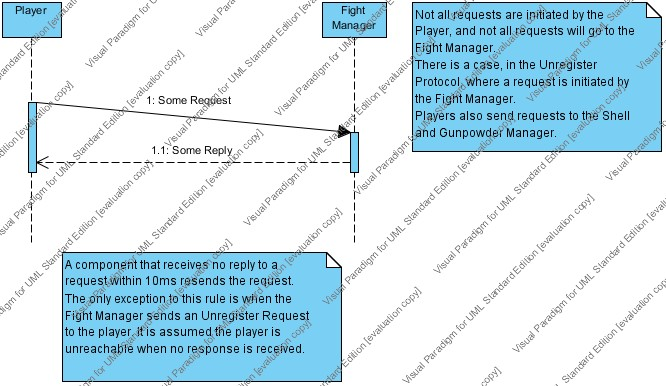
\includegraphics[width=\textwidth]{Diagrams/Sequence Diagrams/General.jpg}
				\caption{Sequence and timing of messages in a general request-reply pattern}
			\end{figure}
		\end{center}
	\newpage
	\begin{comment}
	\subsection{Player List Protocol}
		\begin{center}
			\begin{figure}[htp]
				\centering
				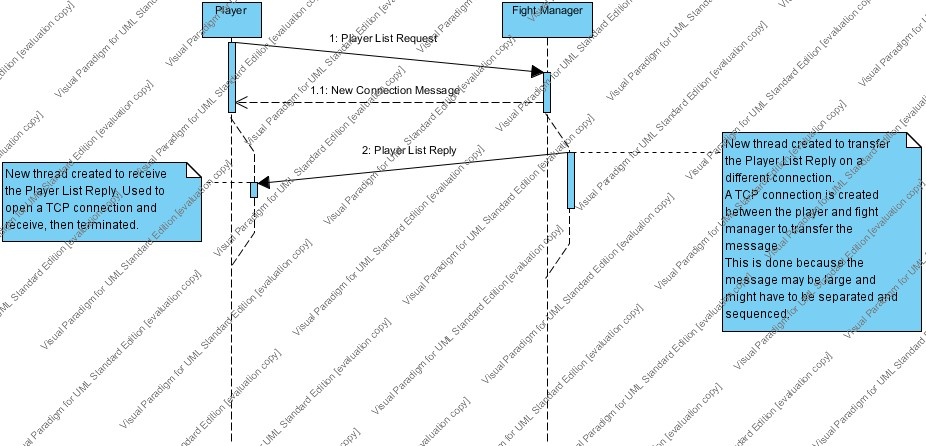
\includegraphics[width=\textwidth]{Diagrams/Sequence Diagrams/Player List Protocol Sequence.jpg}
				\caption{Sequence and timing of messages utilized in the Player List Protocol}
			\end{figure}
		\end{center}
	\newpage
	
	\subsection{Fight List Protocol}
		\begin{center}
			\begin{figure}[htp]
				\centering
				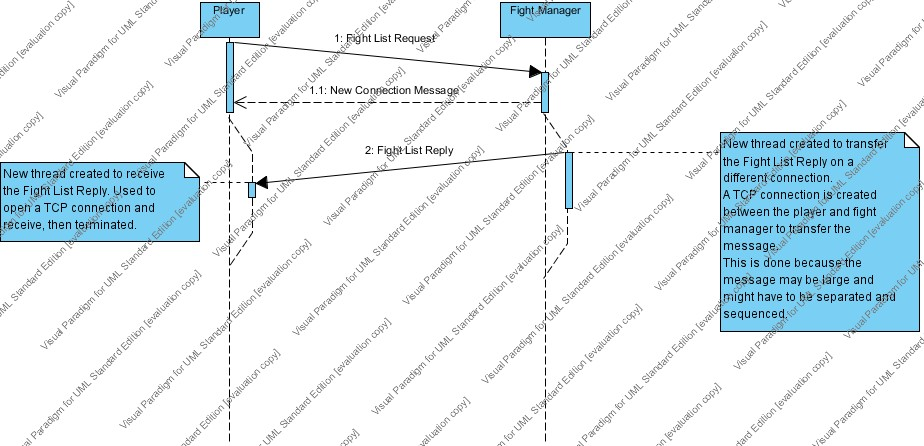
\includegraphics[width=\textwidth]{Diagrams/Sequence Diagrams/Fight List Protocol Sequence.jpg}
				\caption{Sequence and timing of messages utilized in the Fight List Protocol}
			\end{figure}
		\end{center}
	\newpage
	\end{comment}
	\subsection{Location List Protocol}
		\begin{center}
			\begin{figure}[htp]
				\centering
				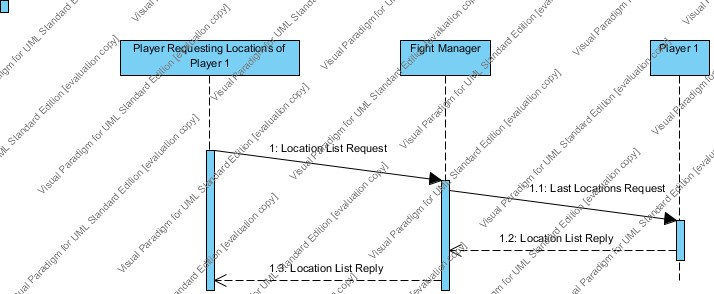
\includegraphics[width=.7\textwidth]{Diagrams/Sequence Diagrams/Location List Protocol Sequence.jpg}
				\caption{Sequence and timing of messages utilized in the Location List Protocol}
			\end{figure}
		\end{center}
	\newpage
	\subsection{Fire Shell Protocol}
		\begin{center}
			\begin{figure}[htp]
				\centering
				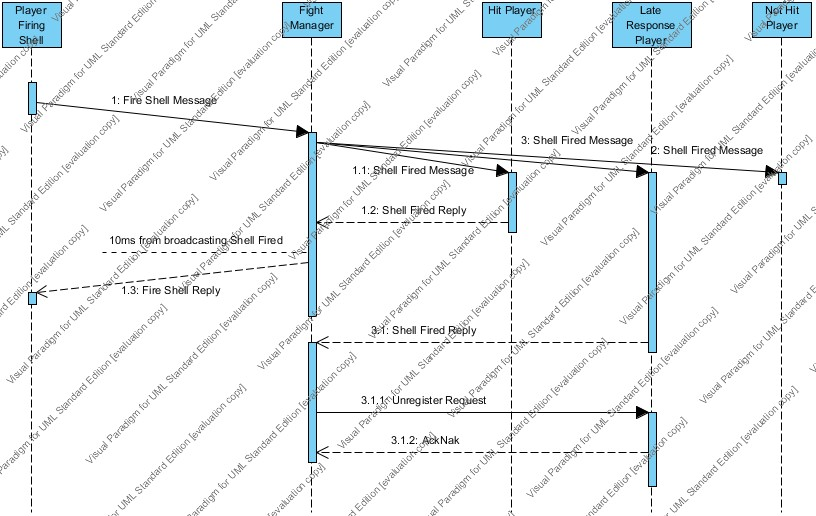
\includegraphics[width=\textwidth]{Diagrams/Sequence Diagrams/Fire Shell Protocol Sequence.jpg}
				\caption{Sequence and timing of messages utilized in the Fire Shell Protocol}
			\end{figure}
		\end{center}
	\newpage
	\subsection{Create Fight Protocol}
		\begin{center}
			\begin{figure}[htp]
				\centering
				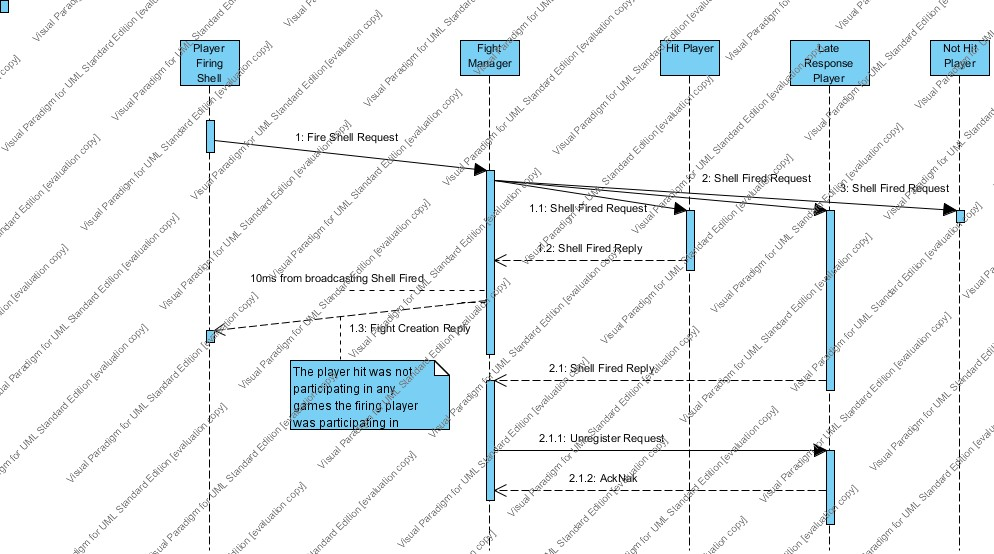
\includegraphics[width=\textwidth]{Diagrams/Sequence Diagrams/Create Fight Protocol Sequence.jpg}
				\caption{Sequence and timing of messages utilized in the Create Fight Protocol}
			\end{figure}
		\end{center}
	\newpage
	\section{Structure}
		\subsection{Introduction}
			Described here is the structure of the needed components in the system, including the:
				\begin{itemize}
					\item{Fight Manager}
					\item{Client}
					\item{Shell Manager}
					\item{Gunpowder Manager}
				\end{itemize}
		\subsection{Classes}
			\subsubsection{Worker Classes}
				\begin{center}
					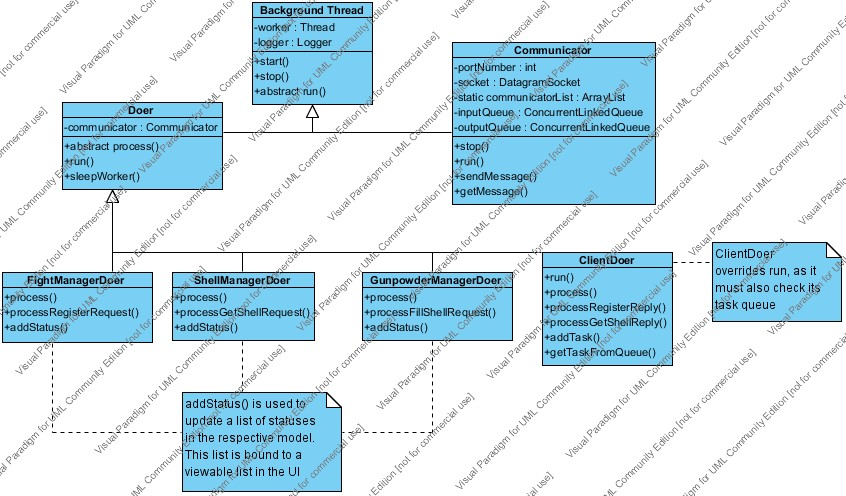
\includegraphics[width=\textwidth]{Diagrams/Structure Diagrams/ThreadingStructure.jpg}
				\end{center}
				\indent Described above are the classes in the system that contain threads that run independent of the main application thread. Each of these classes inherit from BackgroundThread, which describes basic operations inherent to all classes (i.e. start, stop, run). Communicators have a socket that their thread continually tries to receive from. Any received messages are put into an inputqueue, that a Doer can then access. A Doer has a Communicator, and continually checks its inputqueue for new messages. Any messages found are processed by a call to process, and the appropriate action is taken, depending on the type of Doer (FightManager, ShellManager, GunpowderManager, or Client).\\
				All Manager Doers have an addStatus method that updates a list of statuses in the appropriate model. A UI list element is bound to this list, meaning anything added to the list in the model will also appear in the list in the UI.
			\subsubsection{Models and Strategies}
				\begin{center}
					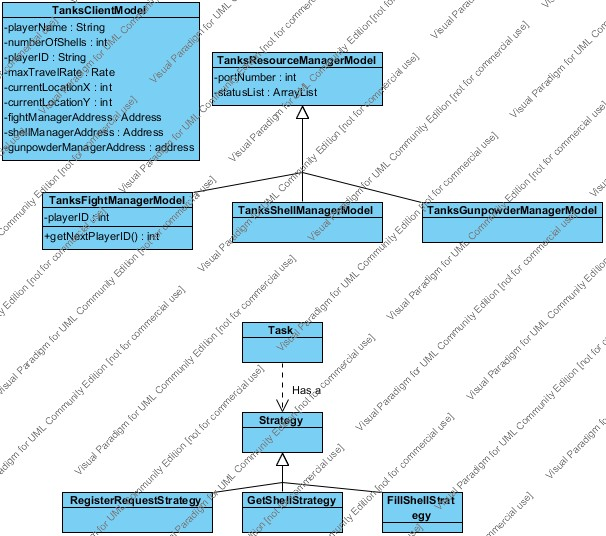
\includegraphics[width=\textwidth]{Diagrams/Structure Diagrams/ModelAndStrategyStructure.jpg}
				\end{center}
				\indent The above diagram depicts both the strategies and models used in the system. 
				\\A model is used to house data about the current state of the application. Things like registered players, player name, player ID, etc. are housed here. In the case of the Managers, the model is only changed and used by their respective Doer. The model used on the client side is used and changed by both the Doer and the Controller. This is done because the UI on the client side is interactive, and the model must change to reflect user choices and entries. 
				\\ Strategies are only used on the client, and are kept within a task. The base class Strategy is abstract, and should not be instantiated. A task is used on the client application when the user has made some action that requires processing by the Doer (this processing usually includes sending message(s) to a manager(s). When this action occurs, a new task is created, along with the correct strategy (i.e. registration, get shell). The Strategy is added to the task, and the task put in the Doer's work queue. The Doer will check this task, and execute the strategy contained within the class.
		\subsection{Components}
			\begin{center}
				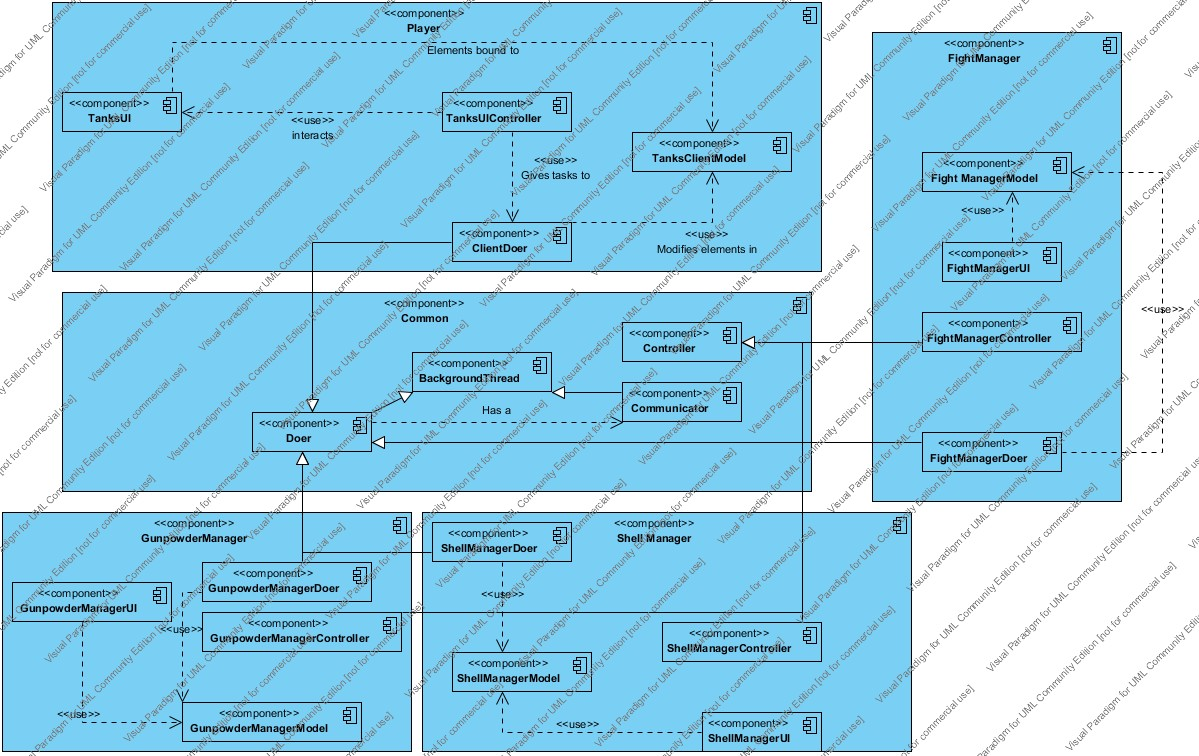
\includegraphics[width=\textwidth]{Diagrams/Structure Diagrams/ComponentDiagram.jpg}
			\end{center}
			\indent The above diagram depicts the components in the system. There are four distinct components in the system:
			\begin{itemize}
				\item{Client: Responsible for responding to player interaction and responding to requests from managers as to the state of the player.}
				\item{Fight Manager: Responsible for tracking players and responding to player requests. Keeps track of certain player stats, and acts as a mediator between players.}
				\item{Shell Manager: Responsible for providing shells to players. These shells are empty, and are not available to be fired until filled.}
				\item{Gunpowder Manager: Responsible for filling shells provided to it. These shells are filled to a specified percentage, and are returned to the player, ready to be fired.}
			\end{itemize} 
			While the above diagram gives a good idea of which components interact with each, it would be best to describe a general sequence of events that happen. When a communicator sees it has received something on its socket, it tries to form a meaningful message from the bytes. Once a message has been reconstituted, it is placed inside of an Envelope(not pictured) that is stamped with the sender and receiver of the message, and put in the communicator's inputqueue. A Doer continually checks its communicator's inputqueue, checking to see if any envelopes are available to process. When an envelope is available, the message is taken out and the type of the message is determined (i.e. registerrequest, getshellrequest). The Doer then calls the appropriate function to handle the type of message. In all cases, data in the model may be updated, or data in the model queried and that data sent back. If the data is to be sent back, the data is put into an appropriate message, which is put into a stamped envelope that is put in the communicator's outputqueue. In the case of the client, any update made to the model is usually reflected in the UI, as UI components are bound to the elements of the model.
		\subsection{Statistics Management}
			As explained in requirement 12, a fight manager must be able to register with and periodically update a webservice with statistics about the current game. The component(s) used in this process are described below.
			\begin{center}
				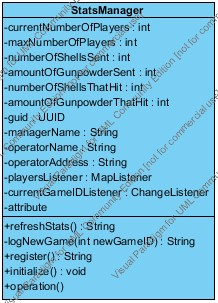
\includegraphics[width=.3\textwidth]{Diagrams/Structure Diagrams/StatsManager.jpg}
			\end{center}
			The attributes and methods of the StatsManager, which is the component that aggregates relevant statistics about the game and may be called to refresh those statistics.
			
			\begin{center}
				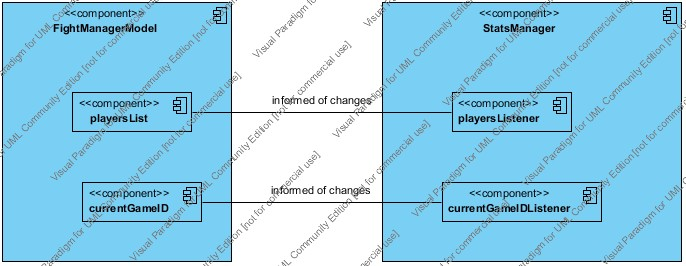
\includegraphics[width=\textwidth]{Diagrams/Structure Diagrams/ComponentDiagram2.jpg}
			\end{center}
			Described above is the general interaction between the FightManagerModel and the StatsManager. It is with this interaction that the StatsManager aggregates and updates its statistics. The attributes playersListener and currentGameIDListener are registered when the StatsManager is initialized to listen to changes in the FightManagerModel. The needed statistics can be determined as the model is changed by the FightManagerDoer, allowing the StatsManager to be a (mostly) hidden entity. The FightManagerDoer must routinely call refreshStats on the StatsManager, but it does so at its own discretion.
\section{Protocol Conversations}
	\subsection{Uniqueness}
		One concern when communicating these protocols across multiple entities is uniquely identifying conversations within an entity. The strategy employed by this system is to have each entity be assigned a unique process ID. All managers are assigned a process ID when they start up, and all players are assigned a unique ID when they register. An entity wishing to start a new protocol conversation selects a number which uniquely identifies that conversation to them. This unique conversation number and the initiating entities' process ID are communicated with every message in the conversation. Any entity can determine which conversation a message corresponds to by looking at the initiating entity and the conversation number unique to that entity.
	\subsection{End Points in a Conversation}
		Another concern is knowing where entities in the system are. This concern is mitigated by a series of progressive steps. As previously described, a client is first known to the system when they register with the fight manager. It is expected in the system that each client knows at startup, without any outside communication, where each manager is located. This allows clients to initiate conversations with every manager. 
		Managers, in order to communicate with clients, track the initiators endpoint in simple request-reply protocols to communicate back to the client. In order to facilitate the communications with clients that did not initiate the conversation, which must occur in the more complex protocols, the fight manager keeps a list of the most recent endpoint used by a client. Whenever the fight manager needs to communicate in this manner, such as when the fight manager must get the last locations of a client, the fight manager uses this list.
	\subsection{Message Tracking}
		For each type of conversation there are specific messages that are expected and that contain information vital to the conversation. An object oriented approach is taken in order to organize messages related to a conversation to some type. An object of a base type Conversation is created and kept for each unique conversation number, process ID combination at every endpoint participating in the conversation. Every protocol described previously within the document has specializations of this base type which allows for the types of messages expected within that conversation to be kept within. In this way each conversation has access to all messages relevant to it.
	\subsection{Message Resends}
		The specialized conversation types also maintain a timer which tracks how long it has been since the last message was sent without a response. A specific time has been determined for every conversation type of when a response is expected. When a timer expires, the original sent message is sent again. These duplicate messages maintain the same identifying message number, conversation number, and process ID that the original did.
		As requests in a conversation may be resent, it is also possible that the receiving endpoint receive duplicate messages. In the case that this message corresponds to an active and available conversation, the conversation simply determines whether to reprocess the message or if a reply to the message needs to be resent. In the case a reply needs to be resent, the same reply message previously sent is resent, without modification to message, conversation, or process number. If a message is received that does not correspond to an active and available conversation, it is determined whether it is old. A message is determined to be old when its conversation number is less than our lowest conversation number in reference to the initiating process ID. If it is old, the message is simply ignored and assumed to have taken much longer than expected to get to this endpoint. If the message is not old, a new conversation is created based on what type of message it is, and the appropriate action taken by that conversation. 
	\subsection{Conversation Completeness}
		Each specialized Conversation type knows the last message expected in a conversation. When a conversation's initiator receives the last message in a protocol and adds it to the conversation, the conversation may then clean itself up by freeing up its memory. Other participants in the conversation are expected to wait a determined amount of time, usually 1 minute, before deletion to ensure the last message they sent was received correctly and that no resends are needed.
\end{document}